\documentclass[10pt]{article}
\usepackage[letterpaper,margin=1in]{geometry}
\usepackage{mathptmx}
\usepackage[mathlines]{lineno}
\usepackage{amsmath,amssymb}
\usepackage{graphicx}
\usepackage{booktabs}
\usepackage{multirow}
\usepackage{array}
\newcolumntype{L}[1]{>{\raggedright\arraybackslash}p{#1}}
\usepackage{xcolor}
\usepackage{algorithm}
\usepackage{algpseudocode}
\usepackage{tikz}
\usetikzlibrary{arrows.meta,positioning,fit,backgrounds,calc}
\usepackage{caption}
\captionsetup{font=small,labelfont=bf}
\usepackage[round,authoryear,sort&compress]{natbib}
\setlength{\bibsep}{2pt}
\usepackage[colorlinks=true,linkcolor=blue!60!black,citecolor=blue!60!black,urlcolor=blue!60!black]{hyperref}
\sloppy
\setlength{\emergencystretch}{3em}
\linenumbers
\title{\bfseries From Embodied Experience to Persistent Experience-Derived State: An Auditable Unified-Graph Architecture and a Preregistered Boundary Analysis of Activation-Based Access}
\author{Kailin Yan\thanks{ORCID: 0009-0009-6762-2684}\\
\small Department of Computer Science, China University of Petroleum-Beijing at Karamay, Karamay, China\\
\small \texttt{2024015943@st.cupk.edu.cn}}
\date{}
\begin{document}
\maketitle
\begin{abstract}
Embodied agents accumulate experience far faster than they can write it back as persistent state. We present \textsc{Fascinator} (FAS), a cognitive-architecture prototype in which semantic, episodic, and procedural content share one typed, weighted graph, and experience becomes relational structure through a single evidence-weighted attribution pipeline. In an information-asymmetric beacon task, persistent graph context yields 20/20 completions versus 0/20 without context, an effect fully reproduced by activation-free embedding retrieval (20/20): persistent reuse is supported, activation necessity is not. A context-removal experiment shows persistence itself is causally operative (10/10 versus 0/10 after graph reset, exact McNemar $p{=}0.00195$; failure repetitions 2.8 versus 7.7, one-sided Wilcoxon $p{=}0.00098$), while history and retrieval baselines match or exceed FAS whenever the experience stream stays re-readable. A preregistered mechanism campaign rejects activation's incremental value over flat retrieval ($\Delta$JCG${<}0$, Holm $p{=}1.5\times10^{-9}$, 0/200 reversals), with one parameterized exception: weak-edge, shallow-path shared-hub convergence. A baseline-controlled campaign (508 runs) measures the trade-off: goal resumption in 9/10 versus 0/10 runs, at the cost of 10.5 versus 1.0 repeated failures on invalidated goals. All negative results, audits, and a one-command verifier are archived.
\end{abstract}
\vspace{6pt}
\noindent\textbf{Keywords:} cognitive architecture; knowledge graph; spreading activation; embodied agents; episodic memory; preregistration




\section{Introduction}
\label{sec:intro}

As soon as an embodied agent acts for more than a few minutes, it produces a stream of experience: actions, observations, successes, failures. What happens to that stream separates two classes of system. In one class, experience accumulates as logs---available for reflection prompts or retrieval augmentation, but never re-organized into structure that changes future behavior. In the other, experience is consolidated: concrete episodes give way to general relational knowledge that persists, is re-activated in relevant situations, and measurably participates in later decisions. Whether or not the system's core includes a large language model (LLM), the gap between logs and consolidation is a central engineering problem for long-lived agents.

Existing positions are familiar. Cognitive architectures such as ACT-R~\citep{anderson2004integrated} and Soar~\citep{laird2012soar} consolidate experience through specific mechanisms (chunks, reinforcement) but keep memory stores representationally separate. LLM-based agents~\citep{yao2023react,park2023generative,shinn2023reflexion} typically save experience as text or vectors and reuse it through prompting; consolidation is delegated to the model and is not auditable. A graph offers a middle path: if episodic, semantic, and procedural content share one explicitly typed graph, the write-back of experience---two named layers, continuous Hebbian reinforcement and thresholded structural promotion (terminology note in Section~\ref{sec:arch-wb})---becomes a first-class, auditable operation rather than a side effect of prompting.

This paper reports \textsc{Fascinator} (FAS), a Python prototype built around that idea: a \emph{unified cognitive graph} on which spreading activation~\citep{collins1975spreading} drives attention and candidate generation, an attribution pipeline writes experience back as typed relational structure, and ledger and event-framework channels route stored knowledge into behavior. We deliberately keep two propositions separate throughout:

\begin{itemize}
\item[(a)] \textbf{Persistent relational reuse has behavioral value.} Under information asymmetry---the knowledge needed for a decision exists only in memory, not in the current observation---graph context built from experience changes behavior (beacon task: 20/20 completions vs 0/20 without context).
\item[(b)] \textbf{The necessity of activation is not supported.} The same benefit is fully reproduced by activation-free retrieval (D-flat, 20/20), and a preregistered mechanism campaign rejects activation's incremental value over flat retrieval under all four confirmatory conditions.
\end{itemize}

The contributions are:
\begin{enumerate}
\item \textbf{An auditable unified-graph memory architecture.} Semantic, episodic, and procedural content coexist in one typed weighted graph; experience becomes new relational structure only through a single evidence-weighted write-back channel. Isolation experiments verify the channel (0 vs 13 learned nodes under an identical experience stream), cross-context re-activation (4/12 vs 0/8 vs 0/0 marked nodes), and two consumer channels that measurably flip action selection (Sections~\ref{sec:arch}--\ref{sec:res-persist}).
\item \textbf{A preregistered evaluation protocol with honestly reported negative results.} The campaign testing whether spreading activation adds value over flat retrieval was designed, seeded, and committed before execution; its primary hypothesis was rejected ($\Delta$JCG${<}0$ under all four preregistered conditions, Holm $p{=}1.5\times10^{-9}$, 0/200 reversals), and we report this as a primary result (Section~\ref{sec:res-boundary}).
\item \textbf{A boundary analysis of activation-based access.} The single systematic exception---multi-input convergence through a shared hub (30/30 vs 0/30)---is delimited by an 84-cell parameter sweep over edge weight, input count, and path depth, and complemented by a structural diagnosis of relation-direction semantics (Section~\ref{sec:res-boundary}, \ref{sec:discussion}).
\end{enumerate}

Every number in this paper is traceable to archived run outputs or to the output of the analysis scripts that read them: the headline numbers are regenerated by the one-command verifier shipped with the reproducibility package, and the remainder were checked line by line against the archives (audit trail in the package and in the reproducibility report); the evidentiary standard, the deterministic-sandbox protocol, and the statistics are specified in Section~\ref{sec:method}. Internal codenames, per-family provenance, and full per-experiment data are in the Supplementary Material.

\section{Related Work}
\label{sec:related}

\textbf{Cognitive architectures.} ACT-R~\citep{anderson2004integrated} and Soar~\citep{laird2012soar} treat consolidation as mechanism-specific learning over separate memory stores; OpenCog~\citep{hart2008opencog} shares our atom-space motivation but targets general intelligence rather than auditable consolidation of embodied experience. Episodic-memory theory~\citep{tulving1983elements,baddeley2000episodic} and event segmentation~\citep{zacks2007event,schacter2007remembering} motivate our event-framework channel and attribution window. Spreading activation as an access mechanism goes back to~\citet{collins1975spreading}; attention and working-set selection relate to~\citet{itti2001computational,posner1980orienting,cowan2001magical}.

\textbf{LLM-agent memory.} ReAct~\citep{yao2023react}, Generative Agents~\citep{park2023generative}, Reflexion~\citep{shinn2023reflexion}, and RAG~\citep{lewis2020rag} reuse experience through prompting or vector retrieval; consolidation quality is not separately controllable or auditable. Structured-memory systems come closer: HippoRAG~\citep{gutierrez2024hipporag} and GraphRAG~\citep{edge2024graphrag} organize retrieval over graph-structured indices but do not test activation-based access against flat retrieval on the same structure; MemGPT~\citep{packer2023memgpt} manages tiered memory through function calls rather than a persistent relational graph; Voyager~\citep{wang2023voyager} stores reusable Minecraft skills as generated code, an explicit skill library rather than an auditable graph write-back. FAS uses the LLM only as a budgeted interface for language and never as memory (Section~\ref{sec:arch-llm}); the studied knowledge channels run with the LLM hard-disabled.

\textbf{Relation to our contribution.} To our knowledge, none of these lines reports a preregistered test of whether activation-based access beats flat retrieval on the same structure. Our negative result on that question, and the parameter sweep delimiting the exception, are the paper's methodological core.

\section{Materials and Methods}
\label{sec:arch}

We present the system content-first: the graph, activation, write-back, persistence and consumers, then the LLM boundary.

\subsection{The unified cognitive graph}
\label{sec:arch-graph}
FAS maintains a directed, typed, weighted graph $G=(V,E,W)$. Nodes carry a label $\tau_v$ marking memory role (seven classes---items, recipes, action experiences, changes, events, intentions, gaps---sharing one namespace), a base weight $w_v$, a timestamp, and a runtime activation $a_v\in\mathbb{R}$; each edge $e=(u,v,\rho,w)$ carries a relation type $\rho$ (eight classes: produces, belongs-to, drops, needs, needs-tool, leads-to, involves, results) and a static weight $w\in[-2,2]$; negative weights denote suppression. \emph{There is no separate episodic, skill, or intention store}: goals, events, action patterns, and affect are nodes of the same graph, distinguished only by label and relation type (Fig.~\ref{fig:ontology}). Beside the graph there are only two auxiliary layers---a short-term episodic buffer (capacity 100, for short-horizon integration) and a statistical timeline (the ledger)---which never build structure: the sole structure-writing channel is the attribution pipeline of Section~\ref{sec:arch-wb}. The space split serves lifecycle management only; it does not isolate topology.

\begin{figure}[t]
\centering
\resizebox{\textwidth}{!}{%
\begin{tikzpicture}[
  sp/.style={draw, rounded corners, align=center, inner sep=3.5pt, font=\scriptsize},
  sem/.style={sp, fill=blue!8}, epi/.style={sp, fill=orange!12},
  proc/.style={sp, fill=green!10}, selfst/.style={sp, fill=purple!8}, emo/.style={sp, fill=red!8},
  edgeT/.style={font=\tiny, fill=white, inner sep=1pt},
  typed/.style={-{Latex}, semithick, gray!70}, neg/.style={-{Latex}, thick, red!70, dashed},
  cross/.style={-{Latex}, semithick, blue!60!black},
  corridor/.style={-{Latex}, semithick, blue!60!black, rounded corners=8pt}]
% central graph node
\node[sp, minimum width=4.8cm, minimum height=1.35cm, fill=gray!6, font=\footnotesize, draw=gray!60]
  (G) at (0,0) {Unified cognitive graph $G{=}(V,E,W)$\\ \scriptsize single namespace; shared labels \& relation types\\ \scriptsize \emph{cross-space links are the core capability}};
% semantic cluster (left column)
\node[sem] (rc) at (-4.3,3.4) {recipe\\ \texttt{oak\_planks}};
\node[sem] (it) at (-4.4,2.3) {item\\ \texttt{oak\_log}, \texttt{stick}};
\node[sem] (ch) at (-5.8,1.0) {change\\ \texttt{inventory:oak\_log:}\\ \texttt{count\_increased}};
% episodic (top-right / right)
\node[epi] (ev) at (1.7,3.1) {event\\ \texttt{tree disappeared}};
\node[epi] (ae) at (4.9,1.9) {action experience\\ \texttt{gather(oak\_log)}};
% bottom row
\node[proc] (ac) at (3.0,-2.5) {action skill\\ \texttt{gather\_resource},\\ \texttt{craft\_item}};
\node[selfst] (ci) at (-1.5,-3.0) {intention/gap\\ \texttt{CI\_*}, \texttt{gap:use}};
\node[emo] (em) at (-3.9,-3.2) {affect\\ arousal, stress};
% intra-semantic
\draw[typed] (it) -- node[edgeT, pos=0.30, right]{belongs} (rc);
% cross-space links, corridor-routed (never through G)
\draw[corridor] (rc.north) -- (-4.3,4.15) -- (3.25,4.15) -- (3.25,-1.55) -- (ac.north);
\node[edgeT] at (0.2,4.32){needs};
\draw[corridor] (ae.south) -- (4.9,-4.15) -- (-5.2,-4.15) -- (ch.south);
\node[edgeT] at (-0.4,-4.45){leads-to $w{=}conf$};
\draw[corridor] (it.west) -- (-7.35,2.3) -- (-7.35,-2.3) -- (ac.west);
\node[edgeT] at (-4.0,-2.08){drops};
\draw[cross] (ci) -- node[edgeT, pos=0.3, left]{points-to} (it);
\draw[cross] (ev) -- node[edgeT, pos=0.55, above]{involves} (it);
\draw[cross] (ae) -- node[edgeT, pos=0.72, below]{involves} (it);
\draw[neg] (ev) to[bend left=15] (it);
\node[edgeT, text=red!70] at (-1.3,3.42) {suppress $-w$};
\draw[cross] (em.north) -- node[edgeT, pos=0.45, left]{modulates} (-1.9,-0.72);
\draw[cross] (ac.north) -- node[edgeT, pos=0.5, right]{skill} (2.35,-0.72);
\begin{scope}[on background layer]
\node[draw=blue!30, rounded corners, fit=(it)(rc)(ch), inner sep=3pt] (fsem) {};
\node[draw=orange!40, rounded corners, fit=(ev)(ae), inner sep=3pt] (fepi) {};
\node[draw=green!50, rounded corners, fit=(ac), inner sep=3pt] (fproc) {};
\node[draw=purple!40, rounded corners, fit=(ci), inner sep=3pt] (fself) {};
\end{scope}
\node[font=\scriptsize, blue!60!black, anchor=north east] at ([xshift=-2pt, yshift=-3pt]fsem.south east) {semantic};
\node[font=\scriptsize, orange!70!black, anchor=north] at ([yshift=-3pt]fepi.south) {episodic space};
\node[font=\scriptsize, green!50!black, anchor=north] at ([yshift=-3pt]fproc.south) {procedural space};
\node[font=\scriptsize, purple!60!black, anchor=north] at ([yshift=-3pt]fself.south) {self/intention space};
\end{tikzpicture}}%
\caption{The unified graph ontology (schematic). Seven label classes and eight relation types share one namespace; there is no separate episodic, skill, or intention store. Cross-space links (blue, corridor-routed) are the core capability: the \texttt{leads-to} edge from \texttt{action experience} to \texttt{change} (weight = confidence) is the product of the write-back pipeline (Section~\ref{sec:arch-wb}); \texttt{gap} points to an entity to inject activation; \texttt{event} carries a negative-polarity slot edge (red dashed) suppressing the entity (Section~\ref{sec:arch-persist}).}
\label{fig:ontology}
\end{figure}

\subsection{Cognitive state and spreading activation}
\label{sec:arch-act}
The cognitive state at time $t$ is the activation field $\mathbf{a}(t)$. Inputs (observations, intentions, gap injections) deposit initial energy into the corresponding nodes; each step, every active node $u$ emits to its neighbors
\begin{equation}
\Delta a_{u\rightarrow v}(t) \;=\; a_u(t)\,\cdot\, \tilde w_{uv}\,\cdot\, \beta_{\mathrm{cat}}(\rho)\,\cdot\, g_{\mathrm{rel}}(\rho)\,\Big/\; \textstyle\sum_{v'} \max\big(\tilde w_{uv'},0\big),
\label{eq:spread}
\end{equation}
followed by decay $a_v(t{+}1) = (1-\lambda)\,a_v(t) + \sum_u \Delta a_{u\rightarrow v}(t)$, clamped by per-space maxima (episodic space $a_{\max}{=}3$, global default $5$). Emission follows an ``emit = transfer'' policy: each node's emitted quantity per step (default 1.0) is deducted from itself; source nodes are exempt. This is an engineering choice of short memory, not an energy-conservation law. Negative-weight edges contribute suppressive flow; suppression is issued only when the emitting node's positive-weight total is greater than zero. The emission budget is scaled by a modulatory gain
\begin{equation}
g \;=\; \mathrm{clip}\big(1 + 0.3\,\mathrm{arousal} - 0.15\,\mathrm{stress},\; 0.7,\; 1.6\big),
\label{eq:mod}
\end{equation}
where arousal is derived from affective-node activation and stress from a slow tonic offset. Attention is the Top-$k$ of the field and constitutes input to action selection. Fig.~\ref{fig:act-schematic} sketches activation-based access \emph{side by side with its flat-retrieval comparison}; the schematic builds intuition only---all conclusions are carried by the experiments of Section~\ref{sec:res-boundary}.

\begin{figure}[t]
\centering
\resizebox{\textwidth}{!}{%
\begin{tikzpicture}[
  nd/.style={circle, draw, minimum size=10mm, inner sep=0pt, align=center, font=\scriptsize},
  hub/.style={nd, fill=purple!25}, hot/.style={nd, fill=red!50},
  warm/.style={nd, fill=orange!40}, cool/.style={nd, fill=blue!12},
  annot/.style={align=center, text=black!80, font=\scriptsize},
  flow/.style={-{Latex}, semithick}, flat/.style={-{Latex}, thick, gray!50, dashed},
  inib/.style={-{Latex}, thick, red!70, dashed}]
\node[hot] (a) at (0,2.2) {gap A\\ demand 1}; \node[warm] (x) at (2.0,1.8) {entity a};
\node[hot] (b) at (0,0.0) {gap B\\ demand 2}; \node[warm] (y) at (2.0,0.4) {entity b};
\node[hub] (P) at (3.7,1.1) {shared\\ hub P};
\node[cool] (T) at (5.9,2.0) {target\\ oak\_log};
\node[cool] (rp) at (5.9,0.2) {recipe\\ planks};
\node[cool, draw=gray!60, fill=gray!12] (ev) at (7.7,2.9) {event\\ failure};
\draw[flow] (a) -- (x); \draw[flow] (x) -- (P);
\draw[flow] (b) -- (y); \draw[flow] (y) -- (P);
\draw[flow] (P) -- (rp); \draw[flow] (rp) -- (T);
\draw[inib] (ev) -- (T);
\draw[flat] (-1.35,1.75) -- (-1.35,-0.55) -- (2.5,-0.85) -- (5.35,-0.25);
\node[annot, anchor=east] at (-1.55,1.85) {flat: nearest};
\draw[flat] (0.62,-0.45) -- (2.62,-0.45) -- (4.35,-0.45) -- (5.35,1.60) node[annot, pos=0.20, above, sloped]{Top-1};
\node[annot, align=left, anchor=west] at (0.15,-2.05) {
  Diffusion paths: multi-source input converges via relational structure on hub $P$---downstream convergence (Section~\ref{sec:res-boundary}):\\[-0.5mm]
  \quad $\bullet$ mechanism runs: JCG${>}0$ on 200/200 paired seeds; $\ge$2-input MRR@1${=}1.0$ (hypothesis group)\\[-0.5mm]
  \quad $\bullet$ only systematic positive difference: shared-hub topology, FAS 30/30 \emph{vs} flat 0/30 (single weight $w{=}0.5$ design)\\[-0.5mm]
  Flat path: nearest-neighbor retrieval reaches the target directly---sufficient for ordinary retrieval:\\[-0.5mm]
  \quad $\bullet$ $\Delta$JCG${<}0$ under all 4 preregistered conditions (reverse-direction Holm $p{=}1.5\times10^{-9}$, 0/200 reversals)\\[-0.5mm]
  \quad $\bullet$ wider spread dilutes targets ($\rho{=}{-}0.445$, ${-}0.656$); \emph{not drawn as diffusion-always-wins}.};
\end{tikzpicture}}%
\caption{Spreading activation and flat retrieval side by side. Every numbered claim comes from the archived experiments of Section~\ref{sec:res-boundary}; the figure only builds intuition.}
\label{fig:act-schematic}
\end{figure}

\subsection{Experience attribution and write-back}
\label{sec:arch-wb}
After an action settles, its receipt and the attribution window (8--120\,s of environment time) of observations form candidate action--observation pairs. Repeated pairs aggregate into hypotheses carrying support $s$, contra-evidence $c$, and Laplace confidence $\mathrm{conf}=s/(s+c+2)$. When $s\ge 5$ and $\mathrm{conf}\ge 0.80$, the hypothesis is \emph{promoted} to a typed relation on the graph: a \texttt{leads-to} edge of weight $w=\mathrm{conf}$ from the action node $\mathtt{action:}A(x)$ to the change node $\mathtt{change:}O$,
\begin{equation}
\mathtt{action:}A(x) \;\longrightarrow\; \mathtt{change:}O \qquad (\texttt{leads-to},\; w{=}\mathrm{conf}),
\label{eq:wb}
\end{equation}
and both endpoints are mark-activated. This is how experience becomes \emph{new relational structure}: \texttt{action:}/\texttt{change:} nodes exist only as products of this pipeline. \emph{Terminology note.} This paper distinguishes three operations: \emph{continuous reinforcement} (sub-threshold Hebbian co-activation weight adjustment; mechanism measurements in Sections~\ref{sec:res-psa} and \ref{sec:res-system}), \emph{episodic replay consolidation} (reorganization driven by offline replay, implemented in the intention/replay layer but not behaviorally validated here), and \emph{structural promotion} (the thresholded hypothesis $\rightarrow$ graph write defined in this section). The blanket term ``consolidation'' used in the introduction and related work names the problem-level ideal only; every claim about FAS below is made under the name---and within the evidence scope---of one of these three operations. The same ledger maintains per-action success-rate memories, consumed by action selection as prior bonuses ($\pm0.05$)---the second statistical path from experience to behavior. A third channel encodes discrete events as event-framework nodes with polarity-slot edges (implemented and production-default off; this paper assembles it explicitly, Section~\ref{sec:res-persist}). The algorithm is Algorithm~\ref{alg:wb}.

\begin{algorithm}[t]
\caption{Attribution--write-back: experience to relational knowledge}\label{alg:wb}
\begin{algorithmic}[1]
\Require action--observation stream $(a_t,o_t)$ within the window; ledger $\mathcal{L}$; graph $G$
\State For each action $A_t$, associate observations $O_k$ in the window with its settlement as candidate pairs $(A_t,O_k)$
\State Aggregate by action signature: $s\mathrel{+}=1$ (positive outcome), $c\mathrel{+}=1$ (contra)
\State $\mathrm{conf}=s/(s+c+2)$ (Laplace smoothing)
\If{$s \ge 5$ and $\mathrm{conf} \ge 0.80$}
  \State create \texttt{action:}A, \texttt{change:}O nodes if absent
  \State write edge \texttt{action} $\longrightarrow$ \texttt{change} with relation \texttt{leads-to}, weight $w{=}\mathrm{conf}$; mark both active
\EndIf
\State ledger in parallel maintains per-action success priors $\mathcal{L}.\mathrm{prior}(\mathrm{sig}(A))$ consumed by action selection
\end{algorithmic}
\end{algorithm}

\subsection{Persistence and consumers}
\label{sec:arch-persist}
Knowledge survives episode boundaries by construction (the graph is inherited, not reinitialized); persistence carries two payloads: \emph{structure} and \emph{activation values} are both serialized into the next episode, so ``re-activation across contexts'' is a measurable event. Section~\ref{sec:res-persist} measures that re-activated ($a\ge0.05$) differences are carried exactly by episodic structure connecting shared entities (4/12 vs 0/8 vs 0/0). Snapshot rotation and a shrink guard (save refusal to overwrite a running graph with an empty one) are data-integrity mechanisms, not cognitive content.

Four classes of consumer use the knowledge produced by write-back. \textbf{(a) Ledger channel (production):} candidate action scores are reweighted by ledger success priors ($+0.05$ success / $-0.05$ failure). \textbf{(b) Affect/neuromodulation (production, every tick):} arousal and stress scalars modulate the emission gain via Eq.~\ref{eq:mod}. \textbf{(c) Continuous intentions and replay gating (production):} the continuous-cognition cycle runs graph dynamics every 2.5\,s; intention lifecycle and idle-gated offline experience replay belong here. \textbf{(d) Event framework (experimental assembly, production-default off):} negative events suppress entity activation via polarity-slot edges; the code is production-hardened but disabled by default so that nothing lands on the graph in production; all behavioral evidence comes from experimental assembly. \emph{Experimental layers} (sandbox assembly and the LLM decision head of Section~\ref{sec:method-routing}) never enter the production default path; the run recorder only observes---it never modifies cognitive behavior.

\subsection{The LLM as a budgeted interface}
\label{sec:arch-llm}
FAS uses the LLM for language production, interpretation of unstructured input, and (low-frequency) reflection; it never uses the LLM as memory, nor as the source of the knowledge this paper studies. All subject experiments run under an import-time guard that hard-disables the LLM (zero-LLM contract; any call errors out)---the only exceptions are the explicitly labeled decision-head experiments (Section~\ref{sec:method-routing}).

\subsection{The experience-to-knowledge loop}
\label{sec:arch-loop}
Figure~\ref{fig:loop} gives the full conceptual closed loop: experience $\rightarrow$ attribution $\rightarrow$ evidence-weighted write-back $\rightarrow$ graph $\rightarrow$ activation $\rightarrow$ working set $\rightarrow$ consumers $\rightarrow$ action; language generation, interpretation and reflection are its only LLM calls. Full paragraph: Supplementary Material~S19.12.

\begin{figure}[t]
\centering
\resizebox{\textwidth}{!}{%
\begin{tikzpicture}[
  loop/.style={draw, rounded corners, align=center, inner sep=4pt, font=\footnotesize},
  scaff/.style={draw, rounded corners, align=center, inner sep=3pt, font=\scriptsize, fill=gray!12, dashed},
  flow/.style={-{Latex}, semithick},
  node distance=3.5mm and 6mm]
\node[loop] (env) {embodied interaction\\ \scriptsize \strut actions, observations\strut};
\node[loop, right=of env] (per) {perception intake\\ \scriptsize \strut ingestion, segmentation\strut};
\node[loop, right=of per] (epi) {action--observation fragments\\ \scriptsize \strut attribution window 8--120 s\strut};
\node[loop, right=of epi] (ev) {evidence accumulation\\ \scriptsize \strut support / contra / confidence\strut};
\node[loop, right=of ev] (wb) {relational write-back\\ \scriptsize \strut promotion to graph + mark-active\strut};
\node[loop, below=of wb] (graph) {unified cognitive graph $G{=}(V,E,W)$\\ \scriptsize \strut structure + activation values persist\strut};
\node[loop, below=of graph] (act) {spreading activation\\ \scriptsize \strut decay, gain, suppression, Top-$k$\strut};
\node[loop, below=of act] (cs) {task-relevant cognitive state\\ \scriptsize \strut working set of relevant knowledge\strut};
\node[loop, below=of cs] (beh) {behavior / action selection\\ \scriptsize \strut consumers: ledger, events, affect\strut};
\node[scaff, below left=6mm and 2mm of ev] (s1) {scaffolding: recipe/block tables};
\node[scaff, left=of cs] (s2) {consumers: reward ledger, trial ledger,\\ event framework (production default off)};
\draw[flow] (env) -- (per);
\draw[flow] (per) -- (epi);
\draw[flow] (epi) -- (ev);
\draw[flow] (ev) -- (wb);
\draw[flow] (wb) -- (graph);
\draw[flow] (graph) -- (act);
\draw[flow] (act) -- (cs);
\draw[flow] (cs) -- (beh);
\draw[flow] (beh) -| ([xshift=-6mm]env.south) -- (env.south);
\draw[flow] (s1) -| (ev);
\draw[flow] (s2) -- ([yshift=-2.5pt]cs.west);
\end{tikzpicture}}%
\caption{The FAS conceptual loop: from embodied interaction to reusable relational knowledge, and back to behavior via activation and consumers. Dashed blocks are scaffolding (mechanics tables; the necessary precondition characterized by the zero-prior result, Section~\ref{sec:res-system}) and consumption channels. The LLM's only positions in the loop are language production/interpretation/reflection (Section~\ref{sec:arch-llm}).}
\label{fig:loop}
\end{figure}



\subsection{Evaluation protocol}
\label{sec:method}

\subsubsection{Environment, determinism, and what ``paired seeds'' mean}
\label{sec:method-env}
All experiments run in a deterministic \texttt{SandboxWorld} (a discrete Minecraft-style grid with simulated clock, recipe and block tables, and a pseudo-device bridge) on the production stack with the LLM hard-disabled by import-time guards; the decision-head family (Section~\ref{sec:method-routing}) is the explicit exception. Paired seeds instantiate different random instances of deterministic conditions and therefore quantify directional consistency across instances, not population effects; sample sizes: $n{=}5$ subject experiments, $n{=}20$ beacon and routing, $n{=}50$ mechanism campaign, $n{=}10$ persistent-state, controls and campaign v2. Full paragraph: Supplementary Material~S19.8.

\subsubsection{Preregistration and evidence accounting}
\label{sec:method-prereg}
Mechanism-campaign hypotheses, topologies, seed reservoir, metrics and testing scheme were fixed and committed before execution; deviations are reported as such. Evidence is reported at representational, mechanism and behavioral levels across four protocol layers (Table~\ref{tab:evidence}); no general-capability (``L4'') claim is made anywhere, and ``causal'' means rule-like regularities from temporally ordered action--outcome observations with evidence weights---not interventional identification. Statistical conventions per family appear in Table~\ref{tab:stats}; the full accounting paragraph is in Supplementary Material~S19.8.

\begin{table}[t]
\centering\small
\caption{Evidence levels $\times$ protocol layers (merged scale; used to attribute every claim in this paper).}
\label{tab:evidence}
\begin{tabular}{L{3.2cm}L{4.4cm}L{6.3cm}}
\toprule
 & \textbf{Level of the claim} & \textbf{Layer the evidence comes from} \\
\midrule
L1 representational & learned structure exists and re-activates & production default path (zero-LLM subject behavior) \\
L2 mechanism & measurable activation/ledger dynamics & production mechanism under experimental assembly; mechanism-isolation layer (reference models distilled from production semantics) \\
L3 behavioral & stored knowledge changes action selection & assembled consumer channels; decision-head harness (experimental layer, never attached to production) \\
L4 general capability & --- & \emph{explicitly not claimed anywhere in this paper} \\
\bottomrule
\end{tabular}
\end{table}

\subsubsection{The mechanism-campaign protocol (preregistered)}
\label{sec:method-civ}
The core incremental-value campaign compares spreading activation against a direct-injection baseline, a closed-form flat path-product (B2; a genuine sentence-embedding retriever serves as the beacon control in Section~\ref{sec:res-reuse}), a random-activation equal-energy control and an oracle precheck, on four synthetic topologies ($n{=}50$ paired seeds per confirmatory condition), with JCG (joint convergence gain) as primary metric and one-sided Wilcoxon{+}Holm as the frozen test. The full protocol, B2 definition and ancillary families are in Supplementary Material~S19.1; condition-level numbers in Table~S6.

\subsubsection{LLM decision-head protocol (routing experiments)}
\label{sec:method-routing}
One family places a real LLM at the decision point (single model, temperature 0, one call per decision); menu, environment state, task facts, experience stream and per-decision budget are shared across conditions, and only the pre-decision context differs. The repaired official campaign ran on the production edge-building path with nine fast-fail harness invariants (520/520 runs valid) and is positioned as exploratory. Full condition definitions in Supplementary Material~S19.2.

\subsubsection{Reproducibility}
Fixed seeds; single-process deterministic execution; archived raw runs and content summaries; all regression checks pass at the time of writing (82 pytest tests; 108/108 regression-script checks). Details: Supplementary Material~S19.8.

\begin{table}[t]
\centering\footnotesize
\caption{Statistical conventions, one row per comparison family (full version with implementation locations in Supplementary Material~S18). ``Status'': pre $=$ preregistered; post $=$ post-hoc; desc $=$ descriptive (no test). All $p$ values in this paper are produced by the test named in this table.}
\label{tab:stats}
\begin{tabular}{L{3.0cm}L{3.4cm}L{2.2cm}L{1.1cm}L{2.2cm}L{0.9cm}}
\toprule
\textbf{Family} & \textbf{Test} & \textbf{Sidedness} & \textbf{paired $n$} & \textbf{Correction ($m$)} & \textbf{Status} \\
\midrule
Beacon success (\S5.1) & exact McNemar & two-sided & 20 & none & pre \\
Beacon decisions (\S5.1) & paired Wilcoxon & two-sided & 20 & none & pre \\
Mechanism $\Delta$JCG, C-1--C-4 (\S5.3) & Wilcoxon, normal approx.\ (analytic tail) & one-sided; reported Holm value is the \emph{reverse}-direction tail (preregistered-direction tail ${\approx}1$) & 50 & Holm (4) & pre \\
Mechanism secondary (MRR, JCG${>}0$) (\S5.3) & paired Wilcoxon & two-sided & 50 & none (secondary family) & pre \\
Shared-hub sweep (\S5.3) & exact McNemar; Wilcoxon & two-sided & 30 & none (frozen design) & pre \\
Relation-direction diagnosis (\S5.3) & Wilcoxon (exact) & two-sided & 10 & single declared family (21 tests) & pre \\
Campaign v2 C/I/B (\S5.5) & McNemar; Wilcoxon; descriptive counts & two-sided; B descriptive & 10 & Holm (within experiment) & pre \\
Campaign v2 E2/T (\S5.5) & Wilcoxon (exact) & one-sided (direction fixed at design time; not in protocol v1.0) & 10 / 9 & Holm (within experiment) & post \\
Controls C3/C4 (\S5.6) & exact McNemar; Wilcoxon & two-sided & 10 & Bonferroni (8) & pre \\
Persistent state H1/H3 (\S5.6) & exact McNemar & two-sided & 10 & none (three hypotheses) & pre \\
Persistent state H5 (\S5.6) & Wilcoxon & one-sided & 10 & none & pre \\
Routing (\S5.7) & paired Wilcoxon & two-sided & 20 & Bonferroni (280) & post \\
Cross-episode recombination (\S5.7) & McNemar; Wilcoxon & two-sided; one-sided (greater) & 30 & within experiment & pre \\
Determinism re-run (\S5.4) & agreement counts & --- & 20 & --- & desc \\
Presentation-equivalence revision (\S5.8) & none (stopped at gate; 0 runs) & --- & 0 & --- & post \\
\bottomrule
\end{tabular}
\end{table}

\section{Results}
\label{sec:results}

\subsection{Persistent relational reuse: the information-asymmetric beacon task}
\label{sec:res-reuse}

\emph{Task.} The beacon task operationalizes information asymmetry: the knowledge needed to solve the task exists \emph{only} in experience-written memory, in no input prompt. The target recipe is stripped from all task facts (``closed book''); the crafting menu lists \texttt{craft\_X} only while item X's context is present (menu gating); goal entities are excluded from activation seeding. Four conditions, $n{=}20$ paired seeds, temperature 0, all 80 runs valid: \textbf{fas\_full} (persistent graph + activation context), \textbf{D-noact} (same graph context with activation dynamics disabled), \textbf{D-flat} (flat retrieval without activation aggregation), \textbf{llm\_direct} (no memory context).

\begin{table}[t]
\centering\small
\caption{Beacon task results ($n{=}20$ paired seeds per condition; 80 runs). All numbers from the archived campaign analysis.}
\label{tab:beacon}
\begin{tabular}{L{2.4cm}L{2.0cm}L{3.3cm}L{3.3cm}L{2.5cm}}
\toprule
\textbf{Condition} & \textbf{Completed} & \textbf{Decisions (mean, median)} & \textbf{First action \texttt{gather\_oak\_log}} & \textbf{Contrast} \\
\midrule
fas\_full & 20/20 & 2.15, 2 & 20/20 & vs direct: McNemar $p{=}2\times10^{-6}$ \\
D-flat (embedding retrieval) & 20/20 & 2.1, 2 & 19/20 & vs fas: $p{=}1.0$; decisions Wilcoxon $p{=}0.72$ \\
D-noact & 0/20 & 8.0, 8 & 20/20 & vs fas: McNemar $p{=}2\times10^{-6}$ \\
llm\_direct & 0/20 & 8.0, 8 & 17/20 & --- \\
\bottomrule
\end{tabular}
\end{table}

\emph{Results.} fas\_full completes 20/20; llm\_direct completes 0/20 (McNemar exact $p{=}2\times10^{-6}$; every decision window is used up without unlocking the chain). \textbf{D-noact}---structure present, runtime access absent---fails 0/20: structure alone is not usable access. \textbf{D-flat}---activation-free flat aggregation---fully reproduces the benefit (20/20; decisions mean 2.1 vs 2.15, no statistical difference, Wilcoxon $p{=}0.72$). Table~\ref{tab:beacon} reports the full grid. First-action identity gives a mechanism fingerprint: fas and D-noact both choose \texttt{gather\_oak\_log} 20/20, direct only 17/20---the difference is not in first-action choice but in subsequent unlocking.

Two readings must be kept separate. \textbf{(a) Persistent relational reuse produces behavioral benefit} on a high-noise, recipe-opaque, information-asymmetric task. The 0/20 baselines are, by task design, an \emph{existence verification}: closed-book gating makes the recipe unavailable to context-free conditions by construction, so the fas-vs-direct contrast demonstrates that the pipeline delivers the required knowledge through memory, not that memory context is ``statistically significantly better'' in any population sense. \textbf{(b) The necessity of activation is not supported}: D-flat's complete reproduction joins the mechanism campaign of Section~\ref{sec:res-boundary}---flat retrieval suffices on reachable tasks.

\emph{What kind of retriever is D-flat?} A genuine sentence-embedding retriever (BAAI/bge-small-zh-v1.5) over all graph node identifiers; its enabling condition is verified zero-LLM in Supplementary Material~S6 (target nodes rank 2nd and 4th of 44 across all 20 seeds). Full paragraph: S19.9.

\subsection{Write-back isolation, persistence, and consumption}
\label{sec:res-persist}

\emph{Write-back isolation.} If written-back structure were a rearrangement of injected knowledge, disabling write-back would change nothing. The isolation experiment breaks graph write-back on a single switch: perception, actions, and environment are identical; two lineages practice the same four-step chain for eight rounds in the same world. With write-back off, the final graph contains \textbf{0} learned \texttt{action:}/\texttt{change:} nodes; with write-back on, \textbf{13} (Supplementary Figure~S1a). Sorting the 15 promoted relations of the write-back-on lineage (Supplementary Table~S4): 11 substantive action--effect associations (``mining yields items and removes a block''), 4 degenerate relations (action pointing at its own success event---the promotion rules do not distinguish this class; we report rather than hide it), and 2 substantive pairs polluted by the attribution window (downstream craft effects attributed to the upstream gather). The initial recipe tables know \emph{what can craft what}; \emph{what execution produces} can only be established by doing.

\emph{Cross-context re-activation.} Episode 1 practices the chain in one context; Episode 2 changes the surface context completely (interfering stand, different layout) with a structurally similar goal. Three conditions inherit from Episode 1: full graph (G0), flat-memory control with episodic-space nodes stripped (G1), and a clean graph (G2). Across 5/5 seeds: G0 re-activates \textbf{4 of 12} marked nodes ($a\ge0.05$); G1 \textbf{0 of 8}; G2 has none (Supplementary Figure~S2). The re-activation difference is carried exactly by the episodic event structure connecting shared entities; behavioral metrics are identical across conditions---representational/access-layer differences are separated from the behavior layer.

\emph{Ledger consumption.} After 8 rounds of a three-step chain (7 promoted relations), transfer to a structurally related four-step task with ledger inherited or fresh: 13 vs 16 ticks, first action flipped from curiosity detour to experienced resource, difference exactly on the three shared candidates; 5/5 seeds, both succeed. Full paragraph: S19.9.

\emph{Event-framework consumption.} A negative event encoded on the graph (polarity-slot suppression) measurably flips first-action choice (5/5 controls at tick 9 \emph{vs} tick 6 inhibited), and with real failure receipts it is the only trace of a transient failure the statistical channel never sees; scope (experimental assembly, production default off) and full numbers in Supplementary Material~S19.3.

\subsection{Preregistered boundary analysis of activation-based access}
\label{sec:res-boundary}

\emph{The convergence mechanism genuinely runs.} Multi-input convergence on the graph is real: JCG${>}$0 on \textbf{200/200} paired seeds across the four confirmatory conditions; counterfactual and permutation controls behave as required (Supplementary Material~S7, S19.10).

\emph{Incremental value over flat retrieval: rejected.} Against the closed-form flat path-product (B2), all four preregistered conditions show $\Delta$JCG${<}0$ (median differences ${-}0.402$, ${-}0.402$, ${-}0.784$, ${-}0.782$; paired $n{=}50$ per condition; the frozen implementation's one-sided $p$ is half the two-sided $p$ regardless of direction, so on these all-negative data the reported tail is the \emph{reverse} direction (B2${>}$FAS): $p{=}3.8\times10^{-10}$, Holm ($m{=}4$) $1.5\times10^{-9}$, while the preregistered-direction (FAS${>}$B2) tail is its complement, $p{\approx}1$; effect $r{=}0.615$; seeds where FAS beats flat: \textbf{0/200}). MRR: FAS below B2 (0.0435/0.0426 vs 0.5/0.5 on the two smaller topologies; tie at 1.0 on the two larger). Noise robustness is unsupported: robustness-sweep slope 0.0076 (B2 0.0), AUC 0.0427 vs 0.04. \textbf{H3 is rejected}: under these topologies and information budgets, flat retrieval is no worse than diffusion, and usually better (Table~\ref{tab:boundary}, Fig.~\ref{fig:boundary}a).

\begin{table}[t]
\centering\small
\caption{Preregistered boundary analysis: key mechanism-level numbers. All values are read programmatically from the archived statistics files; full data in Supplementary Material S7--S9.}
\label{tab:boundary}
\begin{tabular}{L{4.2cm}L{6.3cm}L{3.3cm}}
\toprule
\textbf{Test} & \textbf{Numbers} & \textbf{Reading} \\
\midrule
JCG${>}0$ (mechanism runs) & 200/200 paired seeds; medians 0.0977/0.0977/0.2158/0.2177 & convergence mechanism is real \\
$\Delta$JCG (C-1--C-4, preregistered) & ${-}0.402$/${-}0.402$/${-}0.784$/${-}0.782$; reverse-direction Holm $p{=}1.5\times10^{-9}$, $r{=}0.615$, 0/200 reversals & \textbf{H3 rejected} \\
MRR (FAS vs B2, smaller topologies) & 0.0435/0.0426 vs 0.5/0.5 & flat better on reachable tasks \\
Noise robustness & slope 0.0076 vs 0.0; AUC 0.0427 vs 0.04 & no diffusion advantage \\
Shared-hub topology (single weight $w{=}0.5$) & FAS 30/30 vs B2 0/30, B1 0/30, B3 5/30 & the one systematic exception \\
Weight sweep & both methods reach MRR${=}1.0$ together at $w{=}0.7$ & structural threshold, not a FAS advantage \\
Dilution & $\rho(\mathrm{reach},\mathrm{act})$: $-0.445$ (noise), $-0.656$ (distractor) & wider spread, flatter target \\
Shared-hub parameter sweep (84 cells $\times$ 30 seeds) & FAS strictly better in 11 cells (all $w{\le}0.5$, $d{\le}1$); flat strictly better in 9 (all $w{\ge}0.7$, $d{\ge}1$); tie in 64; O3 replication 30/30 vs 0/30 & advantage region: weak edges $\times$ shallow convergence paths \\
\bottomrule
\end{tabular}
\end{table}

\emph{The shared-hub exception, parameterized.} The single systematic positive---multi-input convergence through a shared hub (FAS 30/30 \emph{vs} flat 0/30; single weight $w{=}0.5$)---is delimited by a frozen 84-cell sweep: FAS strictly better in 11 cells (all weak weights $w{\le}0.5$, shallow paths $d{\le}1$), flat strictly better in 9 (all strong weights $w{\ge}0.7$), 64 ties; both methods cross MRR${=}1.0$ together at $w{=}0.7$ (a structural threshold, not a FAS advantage). Full mechanism reading in Supplementary Material~S19.4.

\begin{figure}[t]
\centering
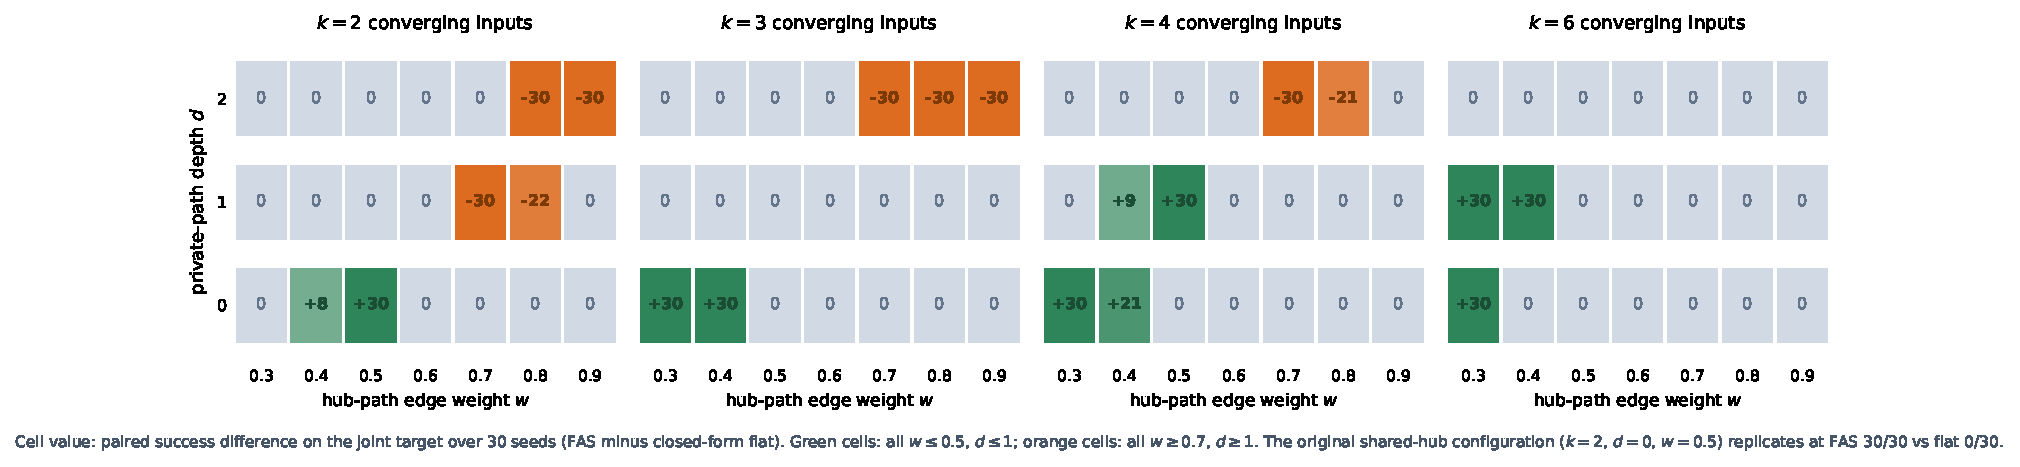
\includegraphics[width=\textwidth]{figures/fig_sweep.pdf}
\caption{Shared-hub parameter sweep (84 cells $\times$ 30 paired seeds, deterministic, zero-LLM). Cell color: paired success difference (FAS minus flat) on the joint target; green = FAS strictly better, orange = flat strictly better, gray = tie; annotations give the cell counts. The FAS-advantage region is confined to weak edge weights and shallow convergence paths. All numbers read programmatically from the archived sweep outputs.}
\label{fig:sweep}
\end{figure}

\begin{figure}[t]
\centering
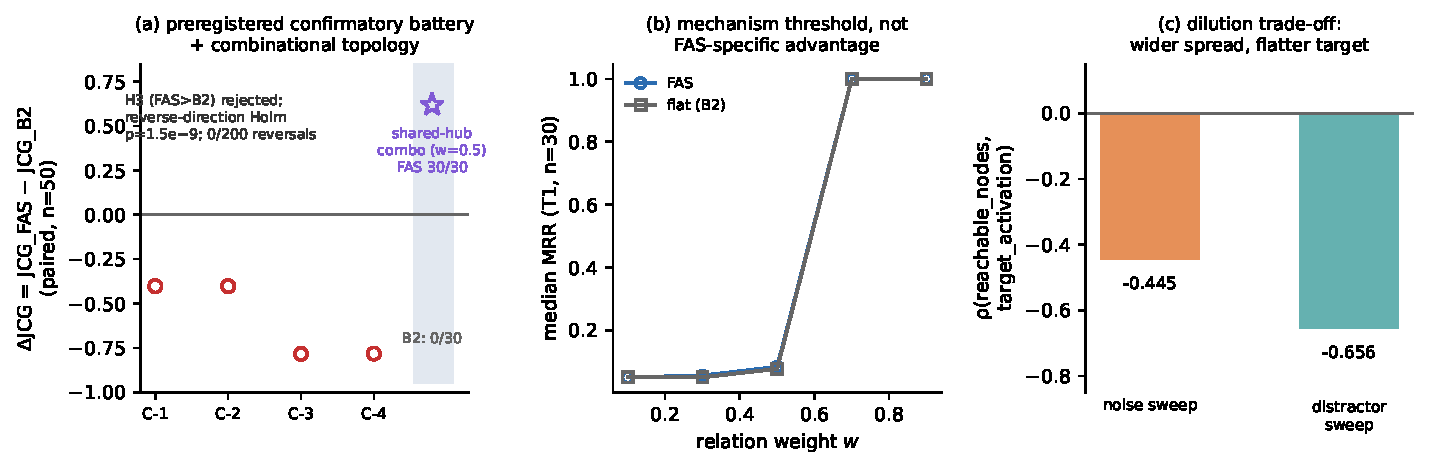
\includegraphics[width=\textwidth]{figures/fig_diffusion_boundary.pdf}
\caption{The diffusion applicability boundary. (a) Preregistered confirmatory family: all four $\Delta$JCG negative (reverse-direction Holm $p{=}1.5\times10^{-9}$); the only positive point is the shared-hub topology (star, single-weight $w{=}0.5$ design). (b) Weight sweep: both methods reach MRR${=}1.0$ together at $w{=}0.7$. (c) Dilution trade-off: the wider the spread, the flatter the target activation ($\rho{=}{-}0.445$, ${-}0.656$).}
\label{fig:boundary}
\end{figure}

\emph{Relation-direction semantics (diagnostic).} The production recipe graph is a depth-1 star forest whose relation targets are all sinks, making forward two-hop propagation structurally impossible; generic reverse projections restore reachability and roughly double the score-activation rank correlation ($\rho$ 0.325${\rightarrow}$0.645; all 21 paired tests at the minimum attainable two-sided $p$ at $n{=}10$) at a dilution cost. Design-level diagnostic, not behavioral evidence; full data in Supplementary Material~S9 and text in S19.4.

\subsection{Determinism re-run of the decision-head family}
\label{sec:res-rerun}
Re-running a 5-seed $\times$ 4-condition beacon subset against the live endpoint reproduces task outcomes 20/20 but full action sequences only 7/20: trajectory-level determinism is claimed for zero-LLM families only. Full paragraph: Supplementary Material~S19.13.

\subsection{Comparative behavioral evidence (campaign v2)}
\label{sec:res-campaign}

The protocol above tests activation against closed-form and embedding
retrieval on \emph{mechanism} metrics. To test the same questions on
\emph{behavior}, we ran a second campaign (508 archived runs; the 390
runs from the two mid-course confound repairs are archived
separately; design and full data in Supplementary
Material~S15--S17) in which every condition shares the same scripted
experience stream, the same menu, the same LLM decision head
(temperature 0), and the same decision budget---only the memory form differs. Experiment codes follow the campaign archive: C goal resumption, E goal revision, E2 event-frame wiring repair, F self-model consumer, I multi-experience convergence, B delayed credit, J long-run stability, T joint measurement; the tasks T1--T3 of the persistent-state experiment (Section~\ref{sec:res-psa}) use a separate numbering (hunger recovery, resumption under context removal, failure repetition after goal invalidation).

\textbf{Goal resumption under neutral instructions (C).} After an
open-book practice phase (obtain \texttt{oak\_planks}) and an unrelated
distractor phase, the test prompt gives no goal at all
(``you have free choice'') and the recipe facts are stripped. FAS
resumes and completes the abandoned goal in \textbf{9/10} paired seeds;
the full-history LLM baseline and the no-memory baseline resume in
\textbf{0/10} (McNemar $p{=}0.0039$; Holm $p{=}0.0117$). This advantage
is regime-dependent: with a longer experience stream that also contains
a failure episode, the full-history baseline matches FAS at 10/10
(below)---the salience advantage holds in the short-history regime.
Mechanism attribution: a zero-experience control reproduces the
same working set (the recipe-closure prior edge
\texttt{oak\_log}$\rightarrow$\texttt{oak\_planks} re-lights the chain
when the raw material is observed), so the effect is
\emph{observation-triggered activation over prior relational
structure}---relational working-set salience---rather than an
intention-lifecycle mechanism.

\textbf{Goal revision is where the same mechanism costs (E).} With an
infeasible target (tool-gated ore), the full-history baseline stops
repeating the failed gather after \textbf{1.0} failures on average and
pivots immediately; FAS repeats it \textbf{10.5} times and pivots in
7/10 runs (late). A joint measurement (below) gives the direction and
magnitude of this cost precisely. The two results are the same coin: state that keeps
a goal salient under distraction also keeps it salient when the
environment invalidates it.

\textbf{Consumer repairs (E2/F).} We then tested whether the failure
and goal states are simply not consumed by the decision context.
Wiring the production event-frame's negative-polarity encoding into
the campaign assembly (failure$\rightarrow$entity edge $w{=}{-}0.8$,
parameters identical to the production config) reduced repeated
failures from 10.5 to \textbf{7.2} (one-sided exact Wilcoxon
$p{=}0.0098$)---statistically significant, but still far above the history baseline's 1.0 repeats; the residual gap is consistent with design-level goal pressure (constant goal text, weak ledger prior)---an attribution that remains untested. Adding a uniform self-graph goal consumer
(\texttt{current\_goal} $\rightarrow$ working set; production default
off) turned the previously bit-identical ON/OFF behavior into a
separation: with the registry cleared, the consumer-on loop re-derives
the abandoned goal in 5/5 seeds and its gathering actions rise from
1.0 to \textbf{6.0} per run. The self-model's ``behavioral
irrelevance'' was a missing-consumer artifact, not a property of the
representation.

\textbf{Behavioral convergence (I), credit horizon (B), stability (J), joint measurement (T).} Convergence fails at every serialization budget (0--2/10 \emph{vs} raw-history 10/10); the 90\,s attribution window is the credit horizon (10/10 up to 80\,s, 0/10 at 160\,s); 100-cycle stability shows bounded growth ($+3.7\%$ nodes) and zero promotion; the joint measurement replicates the wiring effect (12.0$\rightarrow$7.8, one-sided exact $p{=}0.002$, $n{=}9$ valid pairs) with no resumption gain where the prior-edge path is saturated. E2 and T were designed after the E results and are not part of the frozen campaign protocol v1.0 (which specifies A/B/C/E/F/I/K); they are labeled post-hoc throughout, and T additionally serves as an independent replication of the wiring effect. Full paragraphs, the seed-0 endpoint-error exclusion and the T2b corrected-probe account are in Supplementary Material~S19.7.

\subsection{Persistent-state test under context removal}
\label{sec:res-psa}

The campaign above varies only the memory form; the persistent-state
experiment removes the \emph{experience stream itself} from the
decision context to test the behavioral role of persistence directly
(preregistered; design, all conditions, and data in Supplementary
Material~S16). Three tasks: T1 hunger recovery (existence check), T2
goal resumption under context removal (practice a goal, then a fresh
context with recipe facts stripped and only graph-derived content in
the decision context), and T3 failure repetition after the environment
invalidates the goal. Conditions: \textbf{FAS-full} (persistent graph
context), \textbf{FAS-reset} (same stack, graph and activation reset at
the phase boundary), \textbf{B0-direct} (no context), budgeted raw
history \textbf{h128/h512/h2048}, \textbf{B2-rag} (embedding
retrieval), and \textbf{FAS-sham} (node names without experience
edges). Each hypothesis test uses $n{=}10$ paired seeds; same LLM
decision head (temperature 0), same menu and decision budget.

\textbf{Results.} On T2, FAS-full achieves \textbf{10/10}, FAS-reset
\textbf{0/10} and B0-direct \textbf{0/10} (H1/H3: exact McNemar
$p{=}0.00195$---the minimum attainable at $n{=}10$ with all pairs
discordant, evidencing directional consistency only, not effect size).
H5 (T3): mean failure repetitions \textbf{2.8} (FAS-full) \emph{vs}
\textbf{7.7} (FAS-reset), one-sided Wilcoxon $p{=}0.00098$;
B0-direct 11.2; h2048 and B2-rag both 0.0. The three preregistered
hypotheses are reported with raw $p$ values; Bonferroni over the
family ($m{=}3$) leaves all three below $.05$
($0.0059$, $0.0059$, $0.0029$; computed from the frozen analysis
output). Note that the two failure-repetition figures in this paper
come from different assemblies: campaign E's 10.5 \emph{vs} 1.0
(Section~\ref{sec:res-campaign}) predates the event-frame wiring, while
FAS-full here runs with the negative-polarity channel wired at the
assembly layer. Mechanism observation: the
ten prior-closure edges underwent Hebbian continuous reinforcement
during phase~1---a short-range, within-task natural reproduction
(contrasting with the 30-episode whitelisted drift of
Section~\ref{sec:res-system}).

\textbf{What this experiment does not show.} The controls are \emph{empty} controls (reset clears state; direct has no context), so the experiment establishes that persistence \emph{as a whole} is causally operative---not the independent contribution of graph structure or activation; FAS-sham reaches 10/10; the budget curve is non-diagnostic (inventory echo leak); single task family, $n{=}10$. Full enumeration: S19.11.

\subsection{Additional observations}
\label{sec:res-system}
Seven further observations---long chain and zero-prior starvation (0/25 episodes, ledger untouched), Hebbian sub-threshold drift (3 edges, $+0.074$, retrieval ranks bitwise unchanged), scalar affect moving activation but no action metric, intention formation without expression, exploratory routing (one directional positive, $p{=}0.046$ uncorrected, $p{\approx}1$ after the 280-test correction), live-session growth without an established write-back-to-behavior bridge, and closure masking---are reported verbatim in Supplementary Material~S19.5; their headline numbers are cited where used in Sections 5.1--5.6 and the Limitations.

\subsection{Audit-driven corrections and negative results}
\label{sec:audit-negative}
Four methodological corrections are reported as first-class results in Supplementary Material~S19.6: (C) resumption misattribution corrected to observation-triggered prior-edge salience (regime-dependent); (E) the goal-revision deficit traced to an unwired negative-polarity channel (wiring: 10.5$\rightarrow$7.2, one-sided exact $p{=}0.0098$); (F) the self-model's goal state written but read by no production consumer (a uniform consumer separates behavior, gathers 1.0$\rightarrow$6.0); (T3) the control comparison's T3 advantage traced to failure-evidence visibility, with the presentation-equivalent revision stopped at its own preregistered gate. Preserved negative results: convergence fails at all budgets; the credit horizon is 90\,s; no cross-episode behavioral advantage over retrieval; history/RAG match or exceed FAS whenever the experience stream fits their budget.

\section{Discussion}
\label{sec:discussion}

\subsection{What FAS demonstrates}
\textbf{Shown, within the exact scope of this protocol:} (i) under mechanism-level scaffolding, embodied experience converts into relational structure absent from the initial graph and all injected sources (0 vs 13 nodes; 15 promotions); (ii) that structure persists and re-activates in changed contexts (4/12 vs 0/8 vs 0/0); (iii) two named consumers (ledger, event framework) measurably change behavior (13 vs 16 ticks; 5/5 first-action flips); (iv) under information asymmetry, persistent relational reuse yields a large behavioral difference (20/20 vs 0/20), fully reproducible by activation-free embedding retrieval; (v) the convergence mechanism runs (200/200) yet its incremental value over flat retrieval is preregistration-rejected (0/200 reversals), with the shared-hub exception delimited by the 84-cell sweep; (vi) under context removal, persistence as a whole is causally operative on behavior (FAS-full \emph{vs} the graph-reset empty control: T2 10/10 \emph{vs} 0/10, exact McNemar $p{=}0.00195$; T3 failure repeats 2.8 \emph{vs} 7.7, one-sided Wilcoxon $p{=}0.00098$)---shown only against empty controls. \textbf{Not shown:} general intelligence, open-ended learning from scratch, universal superiority over LLM memory systems, causal understanding, universal diffusion benefits, robust routing value, a behavioral Hebbian benefit, or the independent contribution of graph structure and activation over structure-preserving controls (untested: no presentation-equivalent graph control has been realized; Section~\ref{sec:audit-negative}). Each item is accompanied by its evidence or its absence.

\subsection{Why flat retrieval usually suffices---and when it does not}
The negative results organize into a testable conditional statement rather than a slogan. When the task only asks ``retrieve the related thing,'' flat retrieval does the same work at lower complexity (beacon: D-flat 20/20; campaign: $\Delta$JCG${<}0$). The mechanism-level reason is dilution: the wider the diffusion front, the lower the target activation ($\rho{=}{-}0.445$, ${-}0.656$), which also explains why $-$diffusion is faster on the long chain (259 vs 315 ticks). The sweep sharpens the exception into a region: \emph{activation-based access pays when the task requires multi-relation convergence and the relevant edges are too weak for direct ranking to resolve the target} (all 11 FAS-advantage cells have $w{\le}0.5$, $d{\le}1$); with strong edges, flat ranking resolves everything; with deep weak paths, diffusion dilutes faster than the closed-form product decays (all 9 flat-advantage cells). The guarded hypothesis is: \emph{when decision-relevant information is absent from current observation and the task structure requires multi-relation convergence, activation-based access has positive value over flat retrieval; when information is observable or the task is nearest-neighbor, that value is zero or negative.} Four evidence lines meet at this hypothesis---the beacon (information asymmetry), the shared-hub cells (convergence), the rejected campaign (nearest-neighbor), and the routing tasks (observable information)---none of them stamps it alone.

\subsection{The role of scaffolding}
The zero-prior result (0/25 with an untouched ledger) shows scaffolding is not a convenience but a precondition: the goal system locks onto an unreachable target before any attributable experience exists, and the learning channel starves. FAS is therefore \emph{scaffolded grounded} rather than \emph{learning from scratch}: the architecture must provide the mechanisms (attribution window, thresholds, mechanics tables) that make experience readable and writable. This holds for any system that must act before it can learn, and it is both a necessary transformation and a boundary of capability.

\subsection{Why the unified graph matters}
The three functional evidence chains (re-activation carried by episodic structure, exact ledger transfer onto shared candidates, suppression flips through polarity-slot edges) exist because experience, semantics, and action candidates \emph{share one addressable structure}: in separated stores, each coupling would require custom bridging; here they are natural consequences of graph traversal and graph-based activation. The value of the unified graph is of the form \emph{observable consequences}, and the negative results (closure masking, sub-threshold Hebbian drift) delimit what it cannot do: representational changes do not automatically become behavioral changes.

\subsection{Design implication: direction semantics}
The relation-direction diagnostic (Section~\ref{sec:res-boundary}; full data in Supplementary Material~S9) generalizes into an ontology-design rule: \emph{bake per-relation-class direction semantics into the ontology rather than assume propagation will find its way}---recipe-class relations forward, observation-co-occurrence relations bidirectional. On the measured recipe graph (44 nodes/53 edges), forward two-hop reachability is structurally zero because every relation target is a sink; the improvement after adding reverse projections is a design-level verification, not an emergent property.

\subsection{Limitations}
\label{sec:limits}
(1) All experiments run in a deterministic sandbox with synthetic topologies; paired seeds instantiate different random instances, not real-world variance, and all significance statements quantify directional consistency, not population effects. (2) The beacon's 0/20 baselines are existence verifications built into the task design (closed-book gating), not independent statistical findings. (3) Single environment family, single Minecraft-style domain; no third-party benchmarks; no external-environment validation (e.g., a Crafter-style equivalent) was performed. (4) Subject experiments use five deterministic seeds---descriptive statistics only; paired experiments ($n{=}10$, $n{=}20$, $n{=}50$) carry the directional claims with stated corrections. (5) Semantic write-back structure is not consumed by the planner; learned knowledge affects behavior through the ledger, event-framework, and re-activation channels only. (6) Zero-prior conditions test locking, not learning ability. (7) Not implemented: prospective memory, full perception pipeline, symbolic reasoning, RL policy nodes; several implemented mechanisms are not experimentally validated here. (8) Event-framework behavioral results come from experimental assembly of a production-default-off mechanism. (9) Scaffolding dependence is not quantified. (10) Experimental graphs are small (44--1000 nodes); scale limits all mechanism conclusions. (11) Routing tasks are fully observable at decision time and the negative results are conditional on that; token costs and directional differences are exploratory. (12) The mechanism campaign and relation-direction diagnosis are mechanism-level evidence without production behavioral tests; the shared-hub sweep, while preregistered-style and frozen before execution, is still confined to synthetic hub topologies with a closed-form flat surrogate, not an embedding retriever. (13) The beacon is a single task family (craft domain, closed book); cross-task generality of the information-asymmetry benefit is untested. (14) The decision-head families depend on a remote LLM endpoint at temperature 0; bit-level determinism is verified only by re-running (Section~\ref{sec:res-rerun}) (15) The attribution window (90\,s) is a hard credit horizon: delayed consequences beyond it are never assigned (Section~\ref{sec:res-campaign}). (16) The decision-head context serialization drops the temporal narrative of the experience stream; behavioral convergence tasks therefore fail at this interface. (17) The resumption advantage over full-history baselines is regime-dependent (short-history regime only). (18) The persistent-state experiment (Section~\ref{sec:res-psa}; FAS-full vs FAS-reset, 10/0) used a single task family with a 465-token experience stream; its primary McNemar $p{=}0.00195$ is the minimum attainable at $n{=}10$ and reflects directional consistency, not effect size; the budget curve is non-diagnostic because inventory snapshots in the observation lines leak answer-bearing strings into truncated history. (19) FAS-sham (nodes without experience edges) achieves 10/10 on the goal task, indicating that node-name traces plus menu gating suffice at this task surface. (20) On goal completion (T2), no difference is detected between FAS and the flat-store/no-activation controls (10/10 each, $n{=}10$, limited power); FAS-full's T3 advantage over these controls is attributable to failure-evidence visibility (the control implementations exclude failure information from the decision context), so the independent contribution of graph structure or activation is \emph{not} established. A frozen-preregistration revision attempt stopped at its own presentation-equivalence gate (the naive 2-hop rule still truncates the failure evidence), leaving the question untested; the gate also showed that (a) it checked only step-0 contexts over the Phase-1 baseline store, not Phase-3-evolved text, and (b) C1's context carries additional sections (edges/demand/gap/routing; 22 vs 10 lines) that the graph controls lack, so context structure was never fully aligned; answering the question requires a new, independently preregistered design.

\section{Conclusions}
On a unified cognitive graph, with mechanism-level scaffolding, embodied experience becomes new, typed, evidence-weighted relational knowledge: it persists, re-activates across contexts, and reaches behavior through named consumer channels in measurable, deterministic ways. On the information-asymmetric beacon task, persistent relational reuse yields a 20/20 vs 0/20 behavioral difference, fully reproduced without activation. Spreading activation is a real, measurable access mechanism whose incremental value over flat retrieval is preregistration-rejected everywhere except a now-parameterized shared-hub region: weak edges, shallow convergence paths. The context-removal experiment further locates persistence itself as a causal source of behavior (10/0 against the empty control), while the attribution of that effect to graph structure or activation over structure-preserving controls remains open---the audit marks this boundary explicitly, and the gate-stopped revision attempt leaves the question to future, independently preregistered work. The boundaries are equally clear: no-scaffolding learning regimes are never entered; closure-guaranteed tasks mask internal differences; diffusion's footprint is knowledge access, not action selection. We offer the architecture and the protocol---deterministic, zero-LLM, fully archived, with two reported assembly audits and a preregistered rejection---as a substrate for studying when experience becomes knowledge that changes behavior, and we hand over all negative results as part of the map.



% (Acknowledgments section omitted at author's request, 2026-10-06:
%  nothing to acknowledge.)

% ---------------------------------------------------------------------------
% PeerJ declaration block (author-confirmed 2026-10-06)
% ---------------------------------------------------------------------------
\section*{Funding}
The author received no external funding for this work.

\section*{Competing interests}
The author declares no competing interests.

\section*{Author contributions}
Kailin Yan conceived and designed the study, implemented all software and experiments, performed the statistical analysis, prepared the figures and tables, verified the reproducibility of all reported results, and wrote and revised the manuscript.

\section*{Data and code availability}
All experiments are deterministic and fully archived; the complete reproducibility package --- raw run outputs, graph snapshots, statistics files, source code, preregistration records, and a one-command verifier that recomputes the paper's key numbers without an LLM --- is openly available on Zenodo (DOI: 10.5281/zenodo.23196280) under a split license (data, archives, and documentation: CC BY 4.0; source code: MIT). Preregistrations are included in the package (also Supplementary Material S14--S16). LLM decision-head replications require an anonymized endpoint configuration that is not redistributed; they reproduce at the outcome level rather than bit-identical trajectories (Section~\ref{sec:res-rerun}).

\section*{Reporting guidelines}
No established reporting checklist applies to this study: no human or animal subjects were involved, so ARRIVE/PRISMA/STROBE-type guidelines are not used. The practices actually followed were: confirmatory analyses frozen in repository design documents before execution (the mechanism-campaign manifest, the persistent-state and controls preregistrations, and the presentation-equivalence revision with its gate-stopped preflight), deterministic zero-LLM re-runs, and full archiving of raw outputs; these frozen records are repository files shipped with the reproducibility package, not entries on a public registration platform, and they are summarized in Supplementary Material S14--S18.

\section*{Declaration of generative AI use}
During the preparation of this work the author used the following generative AI tools: Claude (Anthropic, web interface), Claude Code (Anthropic), ChatGPT (OpenAI), and the ZCode agentic coding environment (models: Qwen3.8-flash, DeepSeek-4.1, GLM-5.3-flash). These tools were used for code debugging, \LaTeX{} typesetting assistance, and editorial refinement of manuscript text. They were not used to generate the scientific ideas, experimental designs, analyses, or conclusions; all reported numbers were verified by the author against the archived data with the verification scripts shipped in the reproducibility package. The author takes full responsibility for the content of the manuscript.

\bibliographystyle{apalike}
\bibliography{references}

\end{document}
